%
%  /**-------------------------------------------------------------------**
%   **                         Clan Reference Card                       **
%   **-------------------------------------------------------------------**
%   **                         reference_card.tex                        **
%   **-------------------------------------------------------------------**
%   **                  First version : January 13th 2012                **
%   **-------------------------------------------------------------------**/
%

\documentclass[landscape,a4paper]{article}
\usepackage{t1enc,graphicx,verbatim}
\usepackage{multirow,multicol}
\usepackage[centertags]{amsmath}
\usepackage{amsfonts,amsbsy,amssymb}
\usepackage{pifont}
\usepackage{latexsym}
\usepackage{listings}
\usepackage{tikz}
\usepackage{pslatex} % For cooler font\usepackage{soul}
\lstset{language=C}
\usepackage{ulem}


% For decent A4 (sorry for Letter lovers, Clan is a frenchy):
\oddsidemargin 0.05 in
\evensidemargin 0.05 in
\marginparwidth 0.75 in
\voffset -1.4in
\hoffset -0.77in
\textheight 190 mm
\textwidth 284 mm

% ******************************************************************************
% *                             Version Information                            *
% ******************************************************************************
\def\clanversionnumber{0.7.0}
\def\versionnumber{1.0}
\def\year{2012}
\def\month{January}
\def\version{\month\ \year\ v\versionnumber}

% ******************************************************************************
% *                         Les petites choses pratiques.                      *
% ******************************************************************************
%
% 1.  LISTING DE CODE SOURCE
% 1.1 Description
%     Une zone de texte centree ou on place un code source C dont on indique le
%     fichier .c, avec effets syntaxiques pour une excellente lisibilite.
% 1.2 Utilisation
%     \codesource{largeur}{taille_de_police}{./fichier.c}
%     avec largeur en unites de longueur, par exemple 3cm. et taille_de_police
%     une taille comme small, footnotesize, scriptsize selon les besoins.
%     En scriptsize, ne pas depasser les 69 lignes pour tenir sur une page.
% 1.3 Implementation
%     Necessite le package listings et de preciser le langage, par exemple 
%     avec \lstset{language=C} pour le C. 
\def\codesource#1#2#3{\begin{center}\begin{minipage}{#1}
\begin{#2}\lstinputlisting{#3}
\end{#2}\end{minipage}\end{center}}

% 2.  Titre
% 2.1 Description
%     Un joli titre encadre de lignes faisant la longueur de la colonne.
% 1.2 Utilisation
%     \titre{Texte du Titre}
% 1.3 Implementation
\def\titre#1{\begin{center}\hrule\vspace{0.1cm}#1
\vspace{0.07cm}\hrule\end{center}}

% ******************************************************************************
% *                         Fin petites choses pratiques.                      *
% ******************************************************************************

\parindent = 0pt
%\raggedright

% ******************************************************************************
% *                                 Let's go !                                 *
% ******************************************************************************
\begin{document}

\special{landscape}
\pagestyle{empty}
\raggedcolumns
\setlength{\premulticols}{100pt}
\setlength{\multicolsep}{10pt}
\begin{multicols}{3}

% ******************************************************************************
% *                                   Title                                    *
% ******************************************************************************
\begin{center}
\begin{tabular}{cl}
\multirow{2}{*}{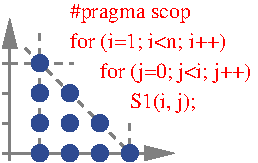
\includegraphics[width=3cm]{images/logo_clan}}
& \\
%& \Large{$\overline{\mbox{\textsc{Clan}}}$ \textsc{Reference \underline{Card}}}\\
& \Large{\textsc{Clan Reference Card}}\\
& \scriptsize{Version \versionnumber\ for Clan \clanversionnumber} \\
&
\end{tabular}
\end{center}

% ******************************************************************************
\titre{About Clan\vspace{0.07cm}}

\begin{small}
Clan is a translator from C-like code parts to polyhedral
representation. It opens the gates of powerful polyhedral compilation
techniques provided by, e.g., PoCC or Pluto. Programmers should ensure their
computation-intensive code parts are compatible with Clan's input to benefit
from state-of-the-art automatic optimization and parallelization.
\end{small}

% ******************************************************************************
\titre{Basic Concepts}

\begin{small}
\textbf{Static Control Parts}\\
Clan is capable to translate program parts easily amenable to the
polyhedral model. We call them \textit{Static Control Parts} (SCoP for short).
They are basically loop-based codes where loop bounds, \texttt{if} conditions and
array subscripts are made of affine expressions involving only outer
loop iterators, integer constants (a.k.a. parameters) and integer literals.

\vspace{0.2cm}
\textbf{SCoP Pragmas}\\
Clan translates code parts delimited by specific pragmas and
ignores what is outside those regions:\\
\ding{229} between {\tt \#pragma scop} and {\tt \#pragma endscop} for C/C++,\\
\ding{229} between {\tt /*@ scop */} and {\tt /*@ end scop */} for JAVA.

\vspace{0.1cm}
In addition to the syntactic restrictions imposed by Clan, inserting
SCoP pragmas in a code also implicitely specifies that:\\
\ding{229} all functions called within the SCoP are pure (no side-effects),\\
\ding{229} no aliasing of array names is possible within the SCoP,\\
\ding{229} pointer references behave like variables or arrays.

\vspace{0.2cm}
\textbf{Affine Expressions}\\
Affine expressions are additive forms of loop iterators (e.g., $i$),
parameters (e.g., $N$) and integers, with integer coefficients, e.g.,
$7*i + 13*N + 42$.\\
\ding{229} Expressions simplifying to affine forms are OK, e.g., $3*(i*2 + N)$.
%\ding{229} Multiplying symbols is \textit{not correct}, e.g.,  $N*i$.

\vspace{0.2cm}
\textbf{Specific Operators}\\
Four particular operators may be used in Clan's input. Let us suppose that
{\tt a} and {\tt b} are affine expressions and {\tt n} an integer:
\vspace{-0.2cm}
\begin{tabbing}
\hskip 205pt \= \kill
Maximum of {\tt a} and {\tt b} ({\tt a} and {\tt b} may be {\tt max} expressions) \> {\tt max(a, b)} \\
Minimum of {\tt a} and {\tt b} ({\tt a} and {\tt b} may be {\tt min} expressions) \> {\tt min(a, b)} \\
Ceil  of {\tt a} divided by {\tt n} (considered as a {\tt max} expression)      \> {\tt ceild(a, n)} \\
Floor of {\tt a} divided by {\tt n} (considered as a {\tt min} expression)      \> {\tt floord(a, n)}
\end{tabbing}
\end{small}

\hrule
\vspace{0.1cm}
\hrule
\begin{scriptsize}
\vspace{0.1cm}
\centerline{\version. Copyright \copyright\ \year\ C\'edric Bastoul and Louis-No\"el Pouchet}

Permission is granted to copy, distribute and/or modify this
document under the terms of the GNU Free Documentation License,
Version 1.2 published by the Free Software Foundation.
Please send comments and corrections to C\'edric Bastoul, \verb+cedric.bastoul@u-psud.fr+

\end{scriptsize}

% ******************************************************************************
\titre{General Restrictions\vspace{0.07cm}}

\begin{small}
Codes between SCoP pragmas must comply to the following restrictions:
\begin{itemize}
\item The only allowed control keywords are {\tt for}, {\tt while}, {\tt if} and
      {\tt else}, with restrictions as described below.
\item Declarations are not allowed.
\item Any C instruction without control keywords is accepted, with
      restrictions for array subscripts as described below.
\end{itemize}
\end{small}

% ******************************************************************************
\titre{Identification of Constrained Elements\vspace{0.07cm}}

\begin{center}
\begin{tikzpicture}
  \node[anchor=south west,inner sep=0] (image) at (0,0) {
    \begin{scriptsize}
    \lstinputlisting{codes/pascal.c}
    \end{scriptsize}
  };
  
  \begin{scope}[x={(image.south east)},y={(image.north west)}]
    \node[draw,rectangle,red,rounded corners=2pt,minimum height=0.3cm,minimum width=0.77cm] (Cond1) at (0.297,0.68){};
    \node[draw,rectangle,red,rounded corners=2pt,minimum height=0.3cm,minimum width=2.39cm] (Cond2) at (0.323,0.605){};
    \node[draw,rectangle,red,rounded corners=2pt,minimum height=0.3cm,minimum width=0.76cm] (Init) at (0.176,0.68){};
    \node[draw,rectangle,red,rounded corners=2pt,minimum height=0.3cm,minimum width=0.47cm] (Step) at (0.402,0.68){};
    \node[draw,rectangle,red,rounded corners=2pt,minimum height=0.3cm,minimum width=0.52cm] (Subs) at (0.559,0.495){};
  
    \coordinate (temp2) at (0.37,0.705);
    \coordinate (temp3) at (0.3,0.755);
    \coordinate (temp4) at (0.18,0.74);
    \node[draw,minimum width=3.2cm] (I) at (0.8,0.9) {\small Loop Initialization};
    \node[draw,minimum width=3.2cm] (C) at (0.8,0.8) {\small Loop and {\tt if} Condition};
    \node[draw,minimum width=3.2cm] (S) at (0.8,0.7) {\small Loop Step};
    \node[draw,minimum width=3.2cm] (A) at (0.8,0.35) {\small Array Subscript};
    \draw[->,>=latex] (I.west) -- (temp3) -- (temp4) -- (Init.north);
    \draw[->,>=latex] (C.west) -- (Cond1.north);
    \draw[->,>=latex] (C.west) -- (temp2) -- (Cond2.27);
    \draw[->,>=latex] (S.west) -- (Step.north east);
    \draw[->,>=latex] (A) -- (Subs);

    % Add this while setting nodes, this is great !
    %\draw[help lines,xstep=.1,ystep=.1] (0,0) grid (1,1);
    %\foreach \x in {0,1,...,9} { \node [anchor=north] at (\x/10,0) {0.\x}; }
    %\foreach \y in {0,1,...,9} { \node [anchor=east] at (0,\y/10) {0.\y}; }
  \end{scope}
\end{tikzpicture}
\end{center}


% ******************************************************************************
\titre{Loop Initialization}

\begin{small}
Each loop initialization must be an assignment of the loop counter such that the
right hand side is one or several affine expressions aggregated with {\tt max}
(resp. {\tt min}) operators if the loop step is positive (resp. negative).
Optionally, the iterator can be declared as an {\tt int} in the initialization part.

\vspace{0.3cm}
\begin{tabular}{p{4cm}|p{4.39cm}}
\multicolumn{1}{c|}{Example of Loop Initialization} &\multicolumn{1}{c}{Diagnostic}\\
\hline
{\tt int j = 3*i + 2*N} & Correct\\
\hline
{\tt j = ceild(i + N, 10)} & Correct if {\tt j} step is positive\\
\hline
{\tt j = max(i, ceild(N, 3))} & Correct if {\tt j} step is positive\\
\hline
{\tt j = min(min(N,10), 7*i)} & Correct if {\tt j} step is negative\\
\hline
\hline
{\tt j = min(max(i, 1), N)} & Incorrect: mixed {\tt min} and {\tt max}
\end{tabular}

\vspace{0.3cm}
\textit{Tip: if the initialization form is too restrictive for a given
program, it may be possible to move the troublesome constraints to the
loop condition or to an external or internal {\tt if} condition.}
\end{small}

% ******************************************************************************
\titre{Loop and {\tt if} Condition}

\begin{small}
Each loop or {\tt if} condition must be a (composition of) constraint(s) on
affine expressions, \sout{and function calls}.
\begin{itemize} %\renewcommand{\labelitemi}{\ding{229}}
\item Supported C operators are {\tt >}, {\tt >=}, {\tt <}, {\tt <=},
      {\tt ==}, {\tt !=}, {\tt !}, {\tt \&\&} and {\tt ||}.
\item {\tt min} and {\tt max} operators can be used to aggregate expressions
      in {\tt >}, {\tt >=}, {\tt <} and {\tt <=} constraints. {\tt min}
      (resp. {\tt max}) expressions must be in the greater (resp. lower)
      side of the constraints.
\item Constraints involving the modulo operator are possible in the following
      form: let {\tt a} be an affine expression and {\tt x} and {\tt y} two
      positive integers, then the condition {\tt (a \% x == y)} is accepted.
\item \sout{Function calls alone can be used as valid {\tt if} conditions}.
\end{itemize}

\vspace{0.3cm}
\begin{tabular}{p{4cm}|p{4.39cm}}
\multicolumn{1}{c|}{Example of Condition} &\multicolumn{1}{c}{Diagnostic}\\
\hline
{\tt i + 2*j < N} & Correct\\
\hline
{\tt max(i, j) < floord(N, 7)} & Correct\\
\hline
{\tt N>i \&\& !(j>0 || N!=1)} & Correct\\
\hline
{\tt ((2*i+1)\%3 == 1) \&\& i>j} & Correct\\
\hline
{\tt func(A[i], b)} & Correct in a {\tt if} condition\\
\hline
\hline
{\tt min(2*i, N) < 0} & Incorrect: {\tt min} on the lower side\\
\hline
{\tt i + 2} & Incorrect: use {\tt (i + 2) != 0}\\
\hline
{\tt i<N \&\& g(a)} & Incorrect: function call not alone
\end{tabular}

\vspace{0.3cm}
\textit{\sout{Tip: to include data-dependent conditions, e.g.,
{\tt if (A[i] == 0)}, create a preprocessor macro containing
the condition and replace it in the SCoP by the macro-function call,
e.g., {\tt if (my\_condition(A[i]))}}}.
\end{small}

% ******************************************************************************
\titre{Loop Step}

\begin{small}
Updating the loop iterator is only allowed in the loop step part.
It must be done by adding an integer to the previous
iterator value. Let {\tt i} be a loop iterator and {\tt x} an integer,
the following forms are accepted for the loop step part:
{\tt i++}, {\tt ++i}, {\tt i---}, {\tt ---i}, {\tt i += x}, {\tt i -= x}, {\tt i = i+x} and
{\tt i = i-x}.
\end{small}

% ******************************************************************************
\titre{Array Subscript}

\begin{small}
Array subscripts must be \sout{either} affine expressions \sout{or function calls}.

\vspace{0.3cm}
\textit{\sout{Tip: to include indirections, e.g., {\tt A[B[i]]}, create a
preprocessor macro containing the subscript and replace it in the SCoP by
the macro-function call, e.g., {\tt A[my\_subscript(B[i])]}}}.
\end{small}

% ******************************************************************************
\titre{Infinite and {\tt while} Loops}

\begin{small}
Infinite {\tt for} loops in the form {\tt for (;;)} are supported.
{\tt while} loops are supported when the condition is \sout{either} {\tt 1}
(infinite loop) \sout{or a function call}.
\end{small}

\end{multicols}

\end{document}
